\documentclass[a4paper,12pt]{article}
\usepackage[top = 2.5cm, bottom = 2.5cm, left = 2.5cm, right = 2.5cm]{geometry} 
\usepackage[T1]{fontenc}
\usepackage[utf8]{inputenc}
\usepackage{multirow} % Multirow is for tables with multiple rows within one cell.
\usepackage{booktabs} % For even nicer tables.

% As we usually want to include some plots (.pdf files) we need a package for that.
\usepackage{graphicx} 
\usepackage{amsmath} % to use split function

% The default setting of LaTeX is to indent new paragraphs. This is useful for articles. But not really nice for homework problem sets. The following command sets the indent to 0.
\usepackage{setspace}
\setlength{\parindent}{0in}

\usepackage{tikz}
%\usetikzlibrary{graphdrawing.trees}


% Package to place figures where you want them.
\usepackage{float}
\usepackage{algorithm} 
\usepackage{algpseudocode} 
% The fancyhdr package let's us create nice headers.
\usepackage{fancyhdr}
\pagestyle{fancy} % With this command we can customize the header style.

\fancyhf{} % This makes sure we do not have other information in our header or footer.

\lhead{\footnotesize Algorithms: Homework 6}% \lhead puts text in the top left corner. \footnotesize sets our font to a smaller size.

%\rhead works just like \lhead (you can also use \chead)
\rhead{\footnotesize Yu-Chieh Kuo} %<---- Fill in your lastnames.

% Similar commands work for the footer (\lfoot, \cfoot and \rfoot).
% We want to put our page number in the center.
\cfoot{\footnotesize \thepage} 

\begin{document}
\thispagestyle{plain} % This command disables the header on the first page. 

\begin{tabular}{p{15.5cm}} % This is a simple tabular environment to align your text nicely 
{\large \bf The Design and Analysis of Algorithms} \\
National Taiwan University, Fall 2020  \\
\hline % \hline produces horizontal lines.
\\
\end{tabular} % Our tabular environment ends here.

\vspace*{0.3cm} % Now we want to add some vertical space in between the line and our title.

\begin{center} % Everything within the center environment is centered.
	{\Large \bf Homework 6} % <---- Don't forget to put in the right number
	\vspace{2mm}
	
        % YOUR NAMES GO HERE
	{\bf Yu-Chieh Kuo B07611039} % <---- Fill in your names here!
		
\end{center}  
\vspace{0.4cm}

This homework answers the problem set sequentially. 

\begin{enumerate}

%problem 1
\item {
We can use divide and conquer method to design the algorithm. For the divide part, we can divide the group into to sub-group, and make them compete with each other; for the conquer part, we make two sub-group play against each other. Let the variable $First$ be the number of the first player, $Last$ be the number of the last player, $Round$ be the total round to schedule, $Result$ be a $n \times (n-1)$ matrix, the algorithm can be written as below.
\begin{algorithm}
	\caption{Round-Robin(First, Last, Round, Result)} 
	\begin{algorithmic}[1]
	    \If{$Last := First +1$}
	        \State Result[$First,Round$] = $Last$
	        \State Result[$Last,Round$] = $First$
	    \Else{}
	        \State $Middle := \frac{First + Last - 1}{2}$
	        \State \textit{//Divide part}
	        \State Round-Robin($First, Middle, \frac{Round+1}{2} - 1$, Result)
	        \State Round-Robin($Middle+1, Last, \frac{Round+1}{2} - 1$, Result)
	        \State \textit{//Conquer part}
	        \For{$i = \frac{Round+1}{2} \ldots Round$}
	            \For{$j = 0 \ldots Middle - First$}
	                \State $Size := \frac{Round+1}{2}$ 
	                \State $Player1 := First + j$
	                \State $Player2 := (Middle + 1) + (i + j) \% size$
	                \State Result[$Player1, i$] = $Player2$
	                \State Result[$Player2, i$] = $Player1$
	            \EndFor
	        \EndFor
	   \EndIf
	\end{algorithmic} 
\end{algorithm}
}

%problem 2
\item{ The graph is as below.

\begin{center}
    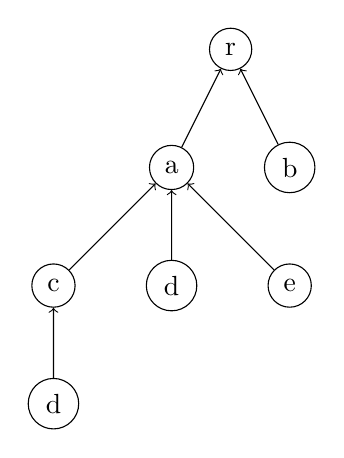
\begin{tikzpicture}[nodes={draw, circle}, <-]
\node{r}
    child { node {a} 
        child { node {c}
            child { node {d} } }
        child { node {d} }
        child { node {e} }
    }
    child { node {b} };
\end{tikzpicture}
\end{center}


}

%problem 3
\item {
The algorithm can be written as below. 
\begin{algorithm}
	\caption{Find(Array)} 
	\begin{algorithmic}[1]
	    \State $n := \text{the length of array}$
	    \State $total := \frac{n(n+1)}{2}$
	    \State $sum := \text{summation of array}$
	    \State \textbf{return} $total - sum$
	\end{algorithmic} 
\end{algorithm}

Since to count the summation of array needs $n$ steps to traverse all array, the time complexity is $\Omega (n)$.

}

%problem 4
\item{
We have already known that the sum of the heights of all nodes in a full binary tree of height $h$ is $2^{h+1} - h - 2$. Let $G(n)$ denote the sum of the heights of all nodes in a complete binary tree with $n$ nodes. For a full binary tree (a special case of complete binary trees) with $n = 2^{h+1} - 1$ nodes where $h$ is the height of the tree, we already know that $G(n) = 2^{h+1} -(h+2) = n-(h+1) \leq n-1$. With this as a basis, we prove the general case of arbitrary complete binary trees by induction on the number $(n \geq 1)$ of nodes. \\
For base case $(n = 1 or n = 2)$: When $n = 1$, the tree is the smallest full binary tree with one single node whose height is $0$. So,$G(n)=0\leq 1-1=n-1$. When $n=2$,the tree has one additional node as the left child of the root. The height of the root is $1$, while that of its left child is $0$. So, $G(n)=1 \leq 2 - 1=n - 1$. \\
For inductive step $(n > 2)$: If $n$ happens to be equal to $2^{h+1} − 1$ for some $h \geq 1, i.e.$ the tree is full, then we are done; note that this covers the case of $n = 3 = 2^{1+1} - 1$. Otherwise, suppose $2^{h+1} - 1 < n < 2^{h+2} - 1 (h \geq 1)$ $i.e.$ the tree is a “proper” complete binary tree with height $h + 1 \geq 2$. We observe that at least one of the two subtrees of the root is full, while the other is complete (possibly full). There are three cases to consider:
\begin{enumerate}
    \item {
The left subtree is full with $n_1$ nodes and the right one is complete but not full with $n_2$ nodes (such that $n_1 + n_2 + 1 = n$). In this case, both subtrees much be of height h and $n_1 = 2^{h+1} - 1$. From the special case of full binary trees and the induction hypothesis, $G(n_1) = 2^{h+1} - (h+2) = n_1 - (h+1)$ and $G(n_2) \leq n_2 - 1$. $G(n) = G(n_1)+G(n_2)+(h+1) \leq (n_1 - (h+1))+(n_2 - 1)+(h+1)=(n_1 +n_2 +1)-2\leq n -1$.
}
    \item {
The left subtree is full with $n_1$ nodes and the right one is also full with $n_2$ nodes. In this case, the left subtree much be of height $h$ and $n_1 = 2^{h+1} - 1$, while the right subtree much be of height $h - 1$ and $n_2 = 2^h - 1$. From the special case of full binary trees, $G(n_1) = 2^{h+1} - (h+2) = n_1 - (h+1)$ and $G(n_2) = 2^h - (h+1) = n_2 - h$. $G(n) = G(n_1)+G(n_2)+(h+1) \leq (n_1 -(h+1))+(n_2 -h)+(h+1) = (n_1 +n_2 +1)-(h+1) \leq n-1$.
}
    \item {
The left subtree is complete but not full with $n_1$ nodes and the right one is full with $n_2$ nodes. In this case, the left subtree much be of height $h$, while the right subtree much be of height $h - 1$ and $n_2 = 2^h - 1$. From the induction hypothesis and the special case of full binary trees, $G(n_1) \leq n_1 -1$ and $G(n_2) = 2^h -(h+1) = n_2 -h$. $G(n) = G(n_1)+G(n_2)+(h+1) \leq (n_1 -1)+(n_2 -h)+(h+1) = (n_1 +n_2 +1)-1 = n-1$.
}
\end{enumerate}

}

%problem 5
\item{ The next function can be adapt as below.
\begin{algorithm}
	\caption{NewNext(B, m, next)} 
	\begin{algorithmic}[1]
	    \For{ $i = 3 \ldots m$}
	        \If{B[next[$i$]+1] == B[$i$]}
	            \State next[$i$] := next[next[$i$] + 1]
	        \EndIf
	    \EndFor
	\end{algorithmic} 
\end{algorithm}
\newpage
The $next$ table will be \\
\begin{center}
\begin{tabular}{ | m | m | m | m | m | m | m | m | m | } 
\hline
1 & 2 & 3 & 4 & 5 & 6 & 7 & 8 & 9 \\
\hline
a & b & a & a & b & a & b & a & a \\ 
\hline
-1 & 0 & -1 & 1 & 0 & -1 & 3 & -1 & 1 \\ 
\hline
\end{tabular}
\end{center}

}

\end{enumerate}

\end{document}
